%; whizzy section -pdf xpdf -latex ./whizzypdfptex.sh
% latex beamer presentation.
% platex, latex-beamer でコンパイルすることを想定。 

%     Tokyo Debian Meeting resources
%     Copyright (C) 2008 Junichi Uekawa

%     This program is free software; you can redistribute it and/or modify
%     it under the terms of the GNU General Public License as published by
%     the Free Software Foundation; either version 2 of the License, or
%     (at your option) any later version.

%     This program is distributed in the hope that it will be useful,
%     but WITHOUT ANY WARRANTY; without even the implied warranty of
%     MERCHANTABILITY or FITNESS FOR A PARTICULAR PURPOSE.  See the
%     GNU General Public License for more details.

%     You should have received a copy of the GNU General Public License
%     along with this program; if not, write to the Free Software
%     Foundation, Inc., 51 Franklin St, Fifth Floor, Boston, MA  02110-1301 USA

\documentclass[cjk,dvipdfmx,12pt]{beamer}
\usetheme{Tokyo}
\usepackage{monthlypresentation}

%  preview (shell-command (concat "evince " (replace-regexp-in-string "tex$" "pdf"(buffer-file-name)) "&"))
%  presentation (shell-command (concat "xpdf -fullscreen " (replace-regexp-in-string "tex$" "pdf"(buffer-file-name)) "&"))

%http://www.naney.org/diki/dk/hyperref.html
%日本語EUC系環境の時
\AtBeginDvi{\special{pdf:tounicode EUC-UCS2}}
%シフトJIS系環境の時
%\AtBeginDvi{\special{pdf:tounicode 90ms-RKSJ-UCS2}}

\title{東京エリア Debian 勉強会}
\subtitle{資料}
\author{岩松 信洋 iwamatsu@debian.or.jp\\IRC nick: iwamatsu}
\date{2008年7月19日}
\logo{
\includegraphics[width=8cm]{image200607/openlogo-light.eps}}

\begin{document}

\frame{\titlepage{}}


\section{Intro}

\emtext{設営準備にご協力ください}

\begin{frame}
 \frametitle{Agenda}
\begin{minipage}[t]{0.45\hsize}
  \begin{itemize}
  \item 注意事項
	\begin{itemize}
	 \item 飲食禁止
	 \item 政治/宗教/営利活動禁止
	\end{itemize}
  \item quiz
  \item 最近のDebian関連のイベント
	\begin{itemize}
	 \item 前回 
	\end{itemize}
 \end{itemize}
\end{minipage} 
\begin{minipage}[t]{0.45\hsize}
 \begin{itemize}
  \item Linux カーネルパッチ パッケージの作り方
  \item Linux ドライバ パッケージの作り方
  \item Debian 温泉
  \item 月刊 kFreeBSD / Nexenta / Hurd / SuperH
 \end{itemize}
\end{minipage}
\end{frame}

\section{最近}


\begin{frame}
 \frametitle{Agenda}
\begin{minipage}[t]{0.45\hsize}
  \begin{itemize}
  \item 注意事項
	\begin{itemize}
	 \item 飲食禁止
	 \item 政治/宗教/営利活動禁止
	\end{itemize}
  \item quiz
  \item 最近のDebian関連のイベント
	\begin{itemize}
	 \item 前回 
	\end{itemize}
 \end{itemize}
\end{minipage} 
\begin{minipage}[t]{0.45\hsize}
 \begin{itemize}
  \item dpatch/debhelperで作成するパッケージ作成方法
  \item Debian GNU/Hurd について熱く語る会
  \item 月刊 kFreeBSD / Nexenta / Hurd / SuperH
  \item OSC 2008 Hokkaido
 \end{itemize}
\end{minipage}
\end{frame}



\section{DWN quiz}
\begin{frame}{Debian 常識クイズ}

Debian の常識、もちろん知ってますよね?
知らないなんて恥ずかしくて、知らないとは言えないあんなことやこんなこと、
みんなで確認してみましょう。

今回の出題範囲は\url{debian-devel-announce@lists.debian.org} に投稿された
内容とDebian Project Newsからです。

\end{frame}

\subsection{問題}

 \santaku
 {Perl 5.10のバグでどのような問題が発生した?}
 {RubyとPythonで書かれたアプリケーションやライブラリがインストールできない}
 {インストールされたファイルのパーミッションが0777になる}
 {特定の名前のファイルがインストールできない}
 {B}% File::Path::rmtreeがツリー削除前にパーミッションを0777にし、それがsymlinkのリンク元にも伝播するようになっていたのが原因。postinstで呼び出されるdebsignがツリーのsymlinkを作成してハッシュを計算した後、この関数を使ってsymlinkを削除しているので、インストール後にファイルのパーミッションが書き換えられる問題に発展した
 
 \santaku
 {Debianプロジェクト内のチームに関する調査で判明した「予想外のチーム」でないものは?}% 調査はDPLのSteve McIntyreが行っている
 {実際に動いているのは1人だけというチーム}
 {誰が作業するか毎回じゃんけんで決めているチーム}
 {お願いやありがとうではなく脅迫で動いているチーム}
 {B}
 
 \santaku
 {wxwidgets2.8がアップロードされたが、長いことwxwidgets2.6の時代が続いていた。その理由は?}
 {パッケージメンテナが保守的で、2.8の使用に対して非積極的だった}
 {アップロードしたところでどうせ誰も使ってくれないとパッケージメンテナが思った}
 {パッケージメンテナが多忙で作業時間がとれなかった}
 {A}% lennyでは2.6をデフォルトとし、2.6で動かないものだけ2.8を使ってほしい、とのこと
 
 \santaku
 {Frans Popの辞任によって、新たな執筆者が求められるようになったものとは?}
 {リリースノート}
 {Debian Project Blog}% Debian Project公式のblog
 {DEB NOTE}% 名前が書かれた開発者を強制的にコミュニティから追い出すノート
 {A}
 
 \subsection{Debian Project News 2008年05号}
 \url{http://www.debian.org/News/weekly/2008/05/}
 にある6月23日版です。
 
 \santaku
 {debian/rulesのget-orig-sourceターゲットは何を記述するためのものか?}
 {「オリジ○弁当」で弁当にソースをつけてもらう方法}
 {upstreamからネットワーク経由でソースコードを取得して現在のソースコードと置き換える方法}
 {upstreamからネットワーク経由で最新の.orig.tar.gzファイルを取得する方法}
 {C}% あまり書かれることのないターゲットだが、skkdicではCVS経由で取得するよう設定している
 
 \santaku
 {リリースゴールに関するPeter Eisentrautの意見は?}
 {リリースゴールなんて所詮一部の開発者の楽しみに過ぎない}
 {Debianの機能の実装に関するリリースゴールはリリース後にポリシーへと変えるべきだ}
 {リリースなんて飾りです。偉い人にはそれがわからんのですよ}
 {B}
 
 \santaku
 {William Pitcockが削除を提案したブートローダパッケージは?}
 {grub}
 {lilo}
 {yaboot}
 {B}% 簡単には直せないgraveなバグがある
 
 \santaku
 {Debian weatherとはどんなサービスか?}
 {特定アーキテクチャのアーカイブの状態を要約して表示する}% その表示に天気の記号を使用している
 {Debian関連ホストが置かれている世界各地の天気を表示する}% worldwideで働いているという意識を高める
 {メーリングリストの流量から世界各地の天気を推測して表示する}% この地域からのメールが多いからこの地域は雨だな、とか
 {A}
 
 \subsection{Debian Project News 2008年06号}
 \url{http://www.debian.org/News/weekly/2008/06/}
 にある7月7日版です。
 
 \santaku
 {Debian 15周年はいつか?}
 {次回の東京エリアDebian勉強会開催予定日である8月16日}
 {本日7月19日}
 {泣く子も黙る7月9日}
 {A}
 
 \santaku
 {Debianのメニュー (.menuファイル) とデスクトップ環境のメニュー (.desktopファイル) に関する議論はどのような結論に落ち着いたか?}
 {freedesktop.orgの.desktopファイルをDebianに合うよう拡張して使っていこう}
 {freedesktop.orgの.desktopファイルには不便な点があるので、働きかけて修正してもらおう}
 {freedesktop.orgの.desktopファイルは使えないのでDebianの.menuファイルを使わせよう}
 {A}% .desktopメニューはユーザビリティを目的とするもので単一階層 (サブカテゴリなし) なのに対し、Debianのメニューは完全性を目的とするもので階層を深く掘っている。ちなみに.menuに比べて.desktopのほうがいいという人はかなり多そう
 
 \santaku
 {6月末に初めて誕生したDebian開発者同士の夫婦とは?}
 {Junichi UekawaとKenshi Muto}
 {Meike ReichleとAlexander Schmehl}
 {Debra MurdockとIan Murdock}% 実はDebraさんがDDになり今更ながら結婚、とか
 {B}
 
 \santaku
 {結婚した二人について述べた以下の事項のうち、正しいものは?}
 {最初の贈り物: DebConf5の土産}% 具体的にはDebConf5のTシャツとフィンランドのチョコレート
 {秘密の愛の交換手段: wiki.debian.org}% planet.d.oで交換していたら誰かに書き換えられた
 {婚約の公式発表手段: lists.debian.org}% planet.d.oで発表したら名前を書き換えられた
 {A}


\section{事前課題紹介}
\emtext{事前課題の紹介}
% pre work home work

\begin{frame}{事前課題}
今回の事前課題は
\begin{enumerate}
 \item Debian に取り込んでほしい Linux カーネルパッチ、Linux ドライバを教えてください。
 \item unstable でアップデートされなくて困ってる Debian パッケージ、BTS に登録されているバグのうち、早く直ってほしいバグを挙げてその理由を教えてください。
 \item {\bf ここで開催してくれないかなぁ} という勉強会の開催地をその理由と共に挙げてください (近いから、だけは却下!)。
\end{enumerate}
というものでした。
\end{frame}

\begin{frame}{鈴木 崇文 さん}
たいして需要もありそうでもなく、結構不安定だという話なので、個人的な趣味の問題ですが、vlookbackというカーネルモジュールが面白いので追加でインストールできるとうれしいです。vloopbackを使用すると、ビデオ出力に手を加えて仮想的なビデオ入力デバイスを通してループバックしたりでき、つまりdv入力をv4lに変換したり、uvcvideoデバイス(v4l2)をv4lに変換できたりしてustream.tvでのストリーミングが使えるようになったりします。
追加モジュールとしてdebパッケージで追加インストールできるのならば、今回の勉強会で学んで試しに自分用のパッケージを作成してみたいです。
\end{frame}

\begin{frame}{前田 耕平さん}
\begin{itemize}
\item {\bf Debian に取り込んでほしい Linux カーネルパッチ、Linux ドライバを教えてください。}
Debianというよりは、LInux自体に対してなんですが、bcm4328がサポートされるとうれしいですね。Broadcomの製品概要を見るとLinuxはサポートOSにはなっているものの、Linux
Wirelessのサイトを見るとまだ対象外\footnote{http://ja.broadcom.com/collateral/pb/4328-PB02-R.pdf}のようです。
先日、Ndiswrapperを使ってようやくMacBookAirで無線LANを利用できるようになったものの、黒MacBookに比べるとどうもIPアドレスの割り当てが不安定です(一度割り当てされると安定するんですが)。
BBモバイルポイントでWEPで接続する分にはまったく問題無かったので、無線LANルータとの相性な気もしなくはないですが。\footnote{http://wireless.kernel.org/en/users/Drivers/b43\#unsupported}
\end{itemize}
\end{frame}

\begin{frame}{前田 耕平さん}
\begin{itemize}
\item {\bf Debian に取り込んでほしい Linux カーネルパッチ、Linux ドライバを教えてください。}
\\
Debianに、という観点では、特定のパッチやドライバというよりは、最新のパッチやドライバ、ソフトウェアのSidへの取り込みがもっと早ければなぁ、と思うことはあります。
Upstreamに比べると遅くなるのは仕方が無いのですが、あまりにかけ離れてしまうと、自分でUpstreamの最新版を持ってきちゃえばいいかと、Debianパッケージは使わずに自分でビルドしてしまうので。
\end{itemize}
\end{frame}

\begin{frame}{前田 耕平さん}
\begin{itemize}
\item {\bf ここで開催してくれないかなぁ という勉強会の開催地をその理由と共に挙げてください (近いから、だけは却下!)。}
\\
割と手頃な値段で借りられそうな候補を上げておきます。
\begin{itemize}
\item 晴海区民館
\url{http://www.city.chuo.lg.jp/sisetugaido/syukaisisetu/syukaisisetu17/}
インターネット接続環境はなし。プロジェクターも無いのがネックです。

\item ITS健保の会議室
半日借りられる、という点では割と安いです。プロジェクターは借りられます。
また、ITSの健保組合員がいないと借りられません。
\end{itemize}
\end{itemize}
\end{frame}

\begin{frame}{前田 耕平さん}
\begin{itemize}
\item {\bf ここで開催してくれないかなぁ という勉強会の開催地をその理由と共に挙げてください (近いから、だけは却下!)。}
\\
\begin{itemize}
\item 市ヶ谷会議室
\url{http://www.its-kenpo.or.jp/restaurant/itigaya_kaigisitu/index.html}
少人数(10人程度)の場合はまぁまぁかも。

\item 山王会議室
\url{http://www.its-kenpo.or.jp/restaurant/sannou_kaigisitu/index.html}
ある程度人数がいないとペイできません。(50人以上)

\item 大久保会議室
\url{http://www.its-kenpo.or.jp/restaurant/okubo_kaigisitu/index.html}
部屋の種類(定員)は一番多いです。

\end{itemize}
\end{itemize}
\end{frame}

\begin{frame}{やまねさん}
\begin{itemize}
\item {\bf BTS に登録されているバグのうち、早く直ってほしいバグを挙げてその理由を教えてください。}
\\
最近はバグウォッチしてないのでなんともむずかしいですが、自分が登録してる
ITP バグをクローズしたいなーとは日々思っています。思ってるだけで何もして
ないんですが。あとは l10n な ja.po は登録して1年とか放置されると悲しい
気分になるので早めにお願いしたい所です(最近はi18nなNMUでfixされますが)。

つーかね、動かねーとか何か変とかいうんだったら、BTS に追加情報だせよゴルァ!
とか思ったりしたりしなかったりする今日この頃。
\end{itemize}
\end{frame}

\begin{frame}{あけどさん}
\begin{itemize}
\item {\bf  unstable でアップデートされなくて困ってる Debian パッケージ、BTSに登録されているバグのうち、早く直ってほしいバグを挙げてその理由を教えてください。}
\\
net-toolsパッケージのいろんなバグ
特にnetstatコマンドのIPv6アドレスが切り落とされるバグは
lenny以降での対応が IPv4 アドレスを表示する形になっていて
ぱっと見ただけで如何にもダメな印象になってしまうので
upstreamを含めて何とかして欲しいところです。

ちなみに他の某ディストリビューションでは
IPv6アドレスが正常に表示されるようになっていて
とても悲しかったりします。

どうやったらプロパーな状況になるんでしょうか?
\end{itemize}
\end{frame}

\begin{frame}{伊藤 弘和さん}
\begin{itemize}
\item {\bf  unstable でアップデートされなくて困ってる Debian パッケージ、BTSに登録されているバグのうち、早く直ってほしいバグを挙げてその理由を教えてください。}

バグというよりは、open-vm-toolsパッケージの修正が一段落ついて欲しいなと思っております。
熱い状態ということもありますが自分も常用している物こそ、貢献できるようになりたいとパッケージの熟成をウォッチしています。
\end{itemize}
\end{frame}

\begin{frame}{大波 誠さん}
\begin{itemize}
\item {\bf Debian に取り込んでほしい Linux カーネルパッチ、Linux ドライバを教えてください。}

正直に申し上げます。パッと思いつくものがありませんでした。ただ、この機会
に「Linux ドライバ」とか「debian ドライバ」とかでぐぐってみました。そした
らThe Linux Foundationがデバイスドライバのオープンソース化を声明として発表
していたり グラフィックボードのドライバなどのプロプライエタリなソフトウェ
アに関する問題が載っていたりして勉強になりました。
前田 耕平さんから勉強会を紹介していただきました。
初参加させていただきます。
\end{itemize}
\end{frame}

\begin{frame}{市川 憲人さん}
\begin{itemize}
\item {\bf  Debianに取り込んで欲しいLinuxカーネルパッチ }

個人的な事情なのですが、自宅サーバがMacBookでそのネット 
ワークインターフェイスが
Marvell Yukon 88E805xで、kernel標準のsky2ドライバ 
はやや挙動が怪しいので、
Marvell提供のドライバをdebianのパッケージ化してあると便 
利です。
自分の技術力ではmake bzImageすら通らなかったので
どなたか技術力のある方がパッケージ化して下さると大変嬉しいです。
\end{itemize}
\end{frame}

\begin{frame}{本庄さん}
\begin{itemize}
\item {\bf Debian に取り込んでほしい Linux カーネルパッチ、Linux ドライバを教えてください。}

特に思いつかないです。

\item {\bf unstable でアップデートされなくて困ってる Debian パッケージ、BTS に登録されているバグのうち、早く直ってほしいバグを挙げてその理由を教えてください。}

アップデートされなくて困っているというわけではありませんが、最近
webminを使いたいと思うことがあり、ちょっと残念でした。

\item {\bf ここで開催してくれないかなぁ という勉強会の開催地をその理由と共に挙げてください (近いから、だけは却下!)。}

以前にも話に上がっていた、温泉宿はどうでしょう。夜を徹して語り合う先になにかが見えるかもしれません。
\end{itemize}
\end{frame}

\begin{frame}{濱野さん}
\begin{itemize}
\item {\bf Debian に取り込んでほしい Linux カーネルパッチ、Linux ドライバを教えてください。}

netfilter の P-O-M patch に含まれる ipset というモジュールを使用してい
ます。なかなか mainstream に入ってくれない様なので package で用意してお
くと便利かな、と思いました。

もうひとつ La Fonera のイメージを触るのに squashfs もあると嬉しいかな、
mksquashfs というユーザランンドツールでこと足りてたりもするのですが\tt\symbol{94}\tt\symbol{94};
\end{itemize}
\end{frame}

\begin{frame}{青木 修}
まあ、かなり利用者の増えているSCIMですがパケージングに参加されている人が
すくないので、なかなかアップデートが追いつきません。

メインのMINGさんは忙しいので、協力してくれるかたいません?私は単なる
UPLOADERで技術的にこれは難しいので、いい人探しています。

あー、開催場所ですが、東工大の長津田キャンパスなどだれか学生さんがいそう
なのになぜないのかなーといつも思っています。
\end{frame}

\begin{frame}{藤沢 理聡 さん}
\begin{itemize}
\item {\bf ここで開催してくれないかなぁ という勉強会の開催地とその理由}

開催地:学校(高校・大学など)
理由:
一言で言うと、学生に興味を持って欲しいからです。
Debianに触れるのに年齢は関係ないと思うけれど、
若いうちにDebianに触れるのも悪くないと思います。
学校という場所や学生という立場では、
今のところLinuxのようなフリーなOSに触れる機会は
多くないのが残念です(社会に出ても触れる機会は多くないけど)。
とにかく、まだ知らない人が興味を持ってくれそうな、
そういう場所で開催するのもいいんじゃないかな、と思いました。
\end{itemize}
\end{frame}

\begin{frame}{岩松 信洋}
\begin{itemize}
\item {\bf Debian に取り込んでほしい Linux カーネルパッチ、Linux ドライバを教えてください。}

今回の資料作成のついでに作りました。内容は発表を参照。

\item {\bf unstable でアップデートされなくて困ってる Debian パッケージ、BTS に登録されているバグのうち、早く直ってほしいバグを挙げてその理由を教えてください。}

kernel-package 関係のバグなど。メンテナ(Manoj)サボリ気味ですね。困りましたね。
libflash の不具合が直ってないのをなんとかしてほしい。

\item {\bf ここで開催してくれないかなぁ という勉強会の開催地をその理由と共に挙げてください (近いから、だけは却下!)。}

先日、東京電機大学さんに行って、コラボできないか相談してきました。学生さんに興味を持たせるにはどうしたらいいですかね。
あとは温泉を8月に企画中です。

\end{itemize}
\end{frame}

% (query-replace "\\subsection" "\\end{frame}\\begin{frame}")
% (query-replace "\\subsubsection" "\\textbf")


% (query-replace "\\subsection" "\\end{frame}\\begin{frame}")
% (query-replace "\\subsubsection" "\\textbf")


\emtext{2008年計画}

\begin{frame}{2008年計画}

{\scriptsize
\begin{enumerate}
 \item 新年会「気合を入れる」
 \item Open Source Conference Tokyo (3/1)
 \item データだけのパッケージを作成してみる、
       ライセンスの考え方 (David Smith)
 \item バイナリ一つのパッケージを作成してみる (吉田@板橋)\\
       バージョン管理ツールを使いDebianパッケージを管理する(git)\\
       アップストリームの扱い(svn/git/cvs)(岩松 信洋さん)
 \item バイナリの分けたパッケージの作成。(前田さん)\\
       バイナリの分け方の考え方、アップグレードなどの運用とか。
 \item パッケージ作成(dpatch/debhelperで作成するパッケージ)(小林儀匡さん)\\
       man の書き方(roff or docbook)(でんさん)\\
       Open Source Conference Hokkaido
 \item パッケージ作成(kernel patch、kernel module)
       、Debconf発表練習
 \item Debconf アルゼンチン、共有ライブラリパッケージ作成

 \item Open Source Conference Tokyo/Fall、
       デーモン系のパッケージの作成、latex、 emacs-lisp、フォントパッケージ
 \item パッケージの cross-compile の方法、amd64 上で i386 のパッケージと
       か、OSC-Fall報告会、Debconf報告会
 \item 国際化 po-debconf / po化 / DDTP
 \item 忘年会
\end{enumerate}
}
\end{frame}
\emtext{Linux カーネルパッチ パッケージの作り方}
\emtext{Linux ドライバ パッケージの作り方}
\emtext{Debian 温泉}
\emtext{月刊 kFreeBSD / Nexenta / Hurd / SuperH /eeepc}

\begin{frame}{宴会場所}
\begin{center}
 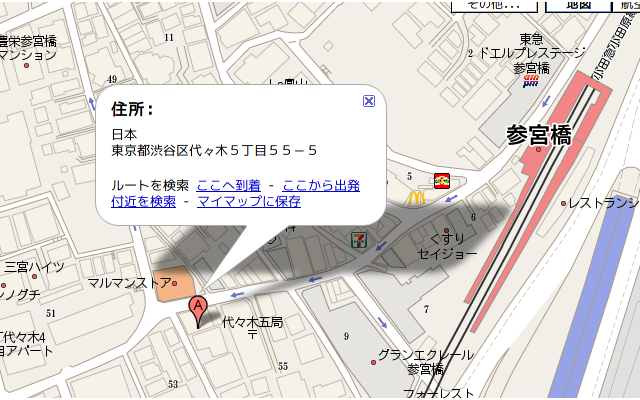
\includegraphics[width=0.7\hsize]{image200806/satsuki.png}
\end{center}

\begin{itemize}
 \item 宴会場所\\
       本日の宴会は「さつき」です。\\
       参加者はフロアに集合し、全員で移動しましょう。
 \item 片付け\\
       部屋を片付けるのにご協力ください。
\end{itemize}

\end{frame}

\end{document}

;;; Local Variables: ***
;;; outline-regexp: "\\([ 	]*\\\\\\(documentstyle\\|documentclass\\|emtext\\|section\\|begin{frame}\\)\\*?[ 	]*[[{]\\|[]+\\)" ***
;;; End: ***
